\selectlanguage{ngerman}
\section{Grundlagen}\label{ch:Grundlagen}
% TODO:
% - Grundsätzlich nötig: Bildsensor (welche technischen Daten nötig), Controller(welche technischen Daten nötig), Speicherung relevanter Daten, Verbindung zwischen Controller und Ausgabegerät (Warum Flutter und Go)
% - Begründete Entscheidung der jeweiligen Hardware und Software (Nennen von Alternativen)
% - Anforderungen an die Objekterkennung (Genauigkeit, Performance)
In diesem Kapitel wird beschrieben, welche Hardware- und Software-Komponenten für die Umsetzung des Projektes nötig sind.
Außerdem wird darauf eingegangen, welche Anforderungen diese erfüllen müssen.

Zunächst wird ein Controller benötigt, welcher genug Rechenleistung aufweist, um die Objekterkennung der Autos umsetzen zu können.
Es wäre Lösung denkbar, bei welcher die Videoaufzeichnungen in eine Cloud gestreamt werden und dort weiterverarbeitet werden. 
Da die Rechenleistung von Controllern für solche Szearien jedoch mittlerweile für eine Objekterkennung stark genug ist und eine direkte Verarbeitung des Videomaterials die Menge der zu übertragenden Datenmengen stark einschränkt, wird ein solches System bevorzugt. 
Dieses benötigt eine Möglichkeit einen Kamera-Sensor anbringen zu können und eine Kommunikationsmöglichkeit über Ethernet oder WLAN.
Die Wahl fällt auf einen Raspberry Pi 3 B+, da dieser bereits vorrätig ist und somit kein zusätzlicher finanzieller Aufwand aufkommt.
Die Rechenleistung ist mit einem 64 bit Quad Core 1.4GHz-Prozessor und 1 GB Arbeitsspeicher für das Projekt ausreichend \cite{pi3}.
Um Autos zu erkennen, wird weder eine hohe Auflösung, noch eine hohe Bildwiederholfrequenz benötigt. 
Es gibt viele Alternativen, welche für die Umsetzung des Projektes denkbar wären.
Beispielsweise sind Mikrocontroller der NVIDIA Jetson- oder der ASUS Tinker Board-Reihe für das Projekt passend \cite{jetson} \cite{tinkerBoard}.

Als Kamera-Sensor wird die Raspberry Pi Camera in der Version 2.1 verwendet. 
Diese wurde speziell für den verwendeten Controller entwickelt und liefert mit einem 8 Megapixel-Sensor eine ausreichende Bildqualität.
Videos können mit bis zu 1080p aufgezeichnet werden \cite{piCAM}.
Der Sensor kann direkt mit dem Controller, über den dafür vorgesehenen seriellen Schnittstellenanschluss, verbunden werden.
Aufgrund der einfachen Kommunikation zwischen Kamera und Controller, sowie einer mehr als ausreichenden Bildqualität wurden als Alternativen lediglich andere Versionen der Pi Camera betrachtet. 

\begin{figure}[h]
	\myImagePos{}
	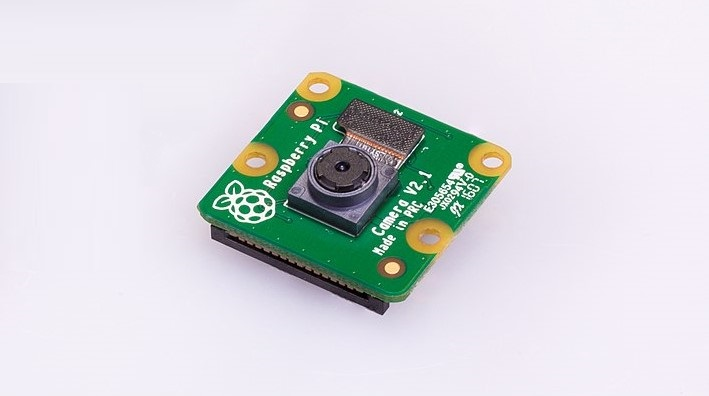
\includegraphics[width=0.4\myImageWidth]{Bilder/piCam.jpg}
	\caption[Raspberry Pi Camera V2.1]{Raspbarry Pi Camera V2.1\cite{PiCamPIC}}
	\label{fig:PiCAM}
\end{figure}

Die Anzeige der Belegung des Parkhauses soll für Studenten und Mitarbeiter der Hochschule Coburg über ein beliebiges Endgerät aus erreichbar sein.
Aus diesem Grund ist es sinnvoll eine Multi-Platform Applikation zu erstellen. 
Diese sollte auf den gängisten Betriebssystemen, wie Android, iOS, Windows oder im Web erreichbar sein.
Diese Anwendungen werden häufig durch Frameworks, wie Flutter, Xamarin oder React Native, realisiert.
Die Wahl des verwendeten Frameworks fällt auf Flutter, da bereits Erfahrungen mit der dessen Programmierung gemacht wurden.
Die Realisierung einer reinen Web-Anwendung wäre ebenfalls möglich gewesen. 
Flutter bietet jedoch die Erstellung von sowohl Internetseiten, als auch Applikationen für verschiedene Betriebssysteme.

Als Bindeglied zwischen Controller und Applikation für den Nutzer muss ein Server für das Handling der Daten implementiert werden.
Die Schnittstelle zum Controller kann über HTTP-Anfragen realisiert werden.
Dieses Konzept ist weit verbreitet und bietet somit einige Frameworks, die für die Umsetzung verwendet werden können.
Für die Schnittstelle zur Applikation ist es sinnvoll, eine Methode zu verwenden, welche es dem Server erlaubt, Daten zu schicken, ohne eine Anfrage zu erhalten.
So kann sichergestellt werden, dass die Anzeige der Anwendung mit dem Auslastungs-Wert des Servers übereinstimmt. 
Ein dafür häufig verwendetes Protokoll ist MQTT.

